\documentclass{beamer}

\usepackage{minted} % For syntax highlighting
\usetheme{metropolis} % Ensure you have the metropolis theme installed

\usepackage{xcolor}
\usepackage{booktabs}
\usepackage{graphicx} % For including images
\usepackage{amsmath}  % For advanced math symbols
\usepackage{tikz}     % For drawing
\usepackage{tcolorbox} % For creating framed blocks
\usetikzlibrary{positioning}

% Define a new tcolorbox style for blocks using Metropolis theme colors
\usecolortheme{metropolis}

\definecolor{mPrimary}{HTML}{005B96} % Primary color for the theme
\definecolor{mSecondary}{HTML}{E37222} % Secondary color for the theme

\tcbset{
    myblock/.style={
        colback=mPrimary!5!white, 
        colframe=mPrimary, 
        fonttitle=\bfseries, 
        title=#1, 
        boxrule=0.5mm, 
        arc=0.5mm, 
        top=1mm, 
        bottom=1mm
    }
}
\definecolor{codebg}{rgb}{0.1,0.1,0.1} % Background color for the code block
\definecolor{codefg}{rgb}{1,1,1} % Foreground color for the code block

% Title and author information
\title{Introduction to Data Mining}
\author{Your Name}
\date{\today}

\begin{document}
\maketitle
\section{Introduction}

% Slide: What is Data Science?
\begin{frame}{What is Data Science}
  \begin{tcolorbox}[myblock={Definition}]
    \scriptsize
    Data science is an interdisciplinary field that uses various techniques and tools to \textbf{analyze} and \textbf{interpret} complex data. It integrates principles from mathematics, statistics, computer science, and domain-specific knowledge to understand and solve real-world problems. Data science involves data cleaning, preparation, advanced modeling, and extracting insights from data to aid \textbf{decision-making} and \textbf{strategic planning}.
  \end{tcolorbox}
  \pause

  \begin{center}
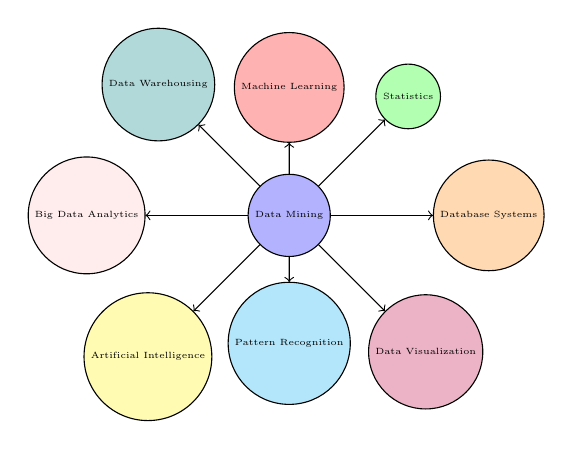
\begin{tikzpicture}[node distance=2.5cm, every node/.style={font=\tiny}, scale=0.65, transform shape]

% Main node
\node[draw, circle, fill=blue!30] (center) {Data Mining};

% Surrounding nodes
\node[draw, circle, fill=red!30] (ml) [above of=center] {Machine Learning};
\node[draw, circle, fill=green!30] (stats) [above right= 1.3cm and 1.3cm of center] {Statistics};
\node[draw, circle, fill=orange!30] (db) [right=2cm of center] {Database Systems};
\node[draw, circle, fill=purple!30] (viz) [below right= 1.3cm and 1.3cm of center] {Data Visualization};
\node[draw, circle, fill=cyan!30] (pr) [below of=center] {Pattern Recognition};
\node[draw, circle, fill=yellow!30] (ai) [below left=1.3cm and 1.3cm of center] {Artificial Intelligence};
\node[draw, circle, fill=pink!30] (ba) [left=2cm of center] {Big Data Analytics};
\node[draw, circle, fill=teal!30] (dw) [above left=1.2cm and 1.2cm of center] {Data Warehousing};

% Connecting lines
\draw[->] (center) -- (ml);
\draw[->] (center) -- (stats);
\draw[->] (center) -- (db);
\draw[->] (center) -- (viz);
\draw[->] (center) -- (pr);
\draw[->] (center) -- (ai);
\draw[->] (center) -- (ba);
\draw[->] (center) -- (dw);

\end{tikzpicture}
\end{center}
\end{frame}
\begin{frame}{What makes a DATA Scientist}
  \begin{itemize}
    \item Uses their data and \alert{analytical} ability to \textbf{find} and \textbf{interpret} rich data sources.\\\pause
    \item Manage \textbf{large amounts} of data.\\\pause
    \item \alert{Create} visualizations to aid in understanding data.\\\pause
    \item \alert{Build Mathematical} models using the data.\\\pause
    \item \alert{Present and communicate} the data insights.
  \end{itemize}
\end{frame}


\section{What is Data}
\begin{frame}{What is Data}
  \begin{center}
    \includegraphics[width=0.7\textwidth]{./whatis_data.jpeg} % Replace with the actual path to your image
  \end{center}
\end{frame}
\begin{frame}{Child Interpretation}
 \begin{table}[]
    \centering
    \begin{tabular}{cccc}
      \toprule
      \textbf{Outlook} & \textbf{Temperature} & \textbf{Windy} & \textbf{Play} \\ 
      \midrule
      sunny   & hot         & no    & no   \\ 
       sunny   & hot         & yes   & no   \\ 
      sunny   & mild        & no    & yes  \\ 
       cloudy  & hot         & no    & yes  \\ 
      rainy   & mild        & no    & yes  \\ 
       rainy   & cold        & yes   & no   \\ 
      \bottomrule
    \end{tabular}
  \end{table}
  \pause
  \begin{itemize}
    \item It's sunny, mild, and windy... \alert{should I play}?
  \end{itemize}
\end{frame}
\begin{frame}[t]
  \frametitle{Features}
  
  \begin{itemize}
    \item \alert{Method 1} :\\[0.5cm]
      \begin{center}
      \begin{tabular}{|c|c|c|c|}
        \hline
        Outlook & Temperature & Windy & Play\\\hline
        1 &  1 & 0 & 0 \\
        \hline
      \end{tabular}
    \end{center}
      \pause
      $$
      F = (1, 1, 0, 1)
      $$
      \pause
    \item \alert{Method 2}: \\[0.3cm]

      \begin{center}
      \begin{tabular}{|c|c|c|c|c|c|c|c|}
        \hline
        Sunny & Cloudy & Rainy & Hot & Mild & Cold & Windy & Play\\\hline
        1 &  0 & 0 & 1 & 0 & 0 & 0 & 0 \\
        \hline
      \end{tabular}
    \end{center}
      $$
      F = (1,0,0, 1,0,0, 0, 0)
      $$

  \end{itemize}

\end{frame}
\begin{frame}[t]
  \frametitle{Measurements}
 
  \vspace*{1cm}

\begin{center}
  \large
  \textbf{Measurements} 
\end{center}

\begin{table}[]
  \centering
  \begin{tabular}{cccccccc}
    \toprule
     &deg & feel & precip. & wsw & uv & thunder \\ 
    \midrule
     &22 & 25 & 13 & 13 & 9 & 0 \\ 
    \bottomrule
    units & ° & ° & \% & km/h & index & \% \\ 
  \end{tabular}
  \caption{Example of data as measurement}
\end{table}
\end{frame}
\begin{frame}[t]
  \frametitle{Others}

  \begin{figure}
  \begin{center}
    \includegraphics[width=0.6\textwidth]{./weather.png} % Replace with the actual path to your image
  \end{center}
  \caption{Weather Measurements}
\end{figure}
\end{frame}

\section{Interpretting Data}%

\begin{frame}[t]
  \frametitle{Back to our basic Example}
\begin{center}
\begin{table}[]
  \centering
  \begin{tabular}{cccc}
    \toprule
    Outlook & Temperature & Windy & Play \\ 
    \midrule
    sunny   & hot         & no    & no   \\ 
    sunny   & hot         & yes   & no   \\ 
    sunny   & mild        & no    & yes  \\ 
    cloudy  & hot         & no    & yes  \\ 
    rainy   & mild        & no    & yes  \\ 
    rainy   & cold        & yes   & no   \\ 
    \bottomrule
  \end{tabular}
\end{table}
\end{center}
\begin{itemize}
  \item Can we think of a set of \alert{rules} to get outside and \textbf{play}?
\end{itemize}

\end{frame}

\begin{frame}[t]
  \frametitle{Rules for Prediction}


  \begin{tcolorbox}[myblock={Objective}]
    \small
    We want to predict our \alert{target} play given the \alert{features} we have available.
  \end{tcolorbox}
 \pause 

 \begin{itemize}
   \item If it's \textbf{Windy} $\longrightarrow$ No play. \\\vspace*{1cm}\pause
   \item If it is \textbf{hot} and \textbf{no wind} $\longrightarrow$ No play.\\\vspace*{1cm}\pause
   \item If it's \textbf{not windy} and \textbf{not hot} $\longrightarrow$ Play
 \end{itemize}
\end{frame}

\begin{frame}[t]
  \frametitle{Formally}
  \framesubtitle{subtitle}

\begin{itemize}
  \item We have our \alert{data} $\mathbf{X}$:
  \begin{itemize}
    \item (with \alert{features:} outlook, temp and windy).
  \end{itemize}
\item Our data consists of smaller \alert{instances}, 'some instance' is written as: $\mathbf{x}$.
  \item If we want to specifically point at a particular instance (say our first row), we write: $\mathbf{x}_1$.
  \item We can see our model as a function $f$, that when given any instance $\mathbf{x}$, gives us a prediction $\hat{y}$.
    $$
    \hat{y} = f(x)
    $$
  \item The application of the model to some instance in our data can be written as $f(\mathbf{x}) = \hat{y}$.
  \item Our hope is that $\hat{y}$ is the same as our \alert{target}: $y$.
\end{itemize}
  
\end{frame}

\begin{frame}[t]
  \frametitle{Recapitulation}
\begin{itemize}
  \item Features $\mathbf{X}$: 
  \begin{itemize}
    \item (outlook, temp., windy)
  \end{itemize}
  \item Target: 
  \begin{itemize}
    \item (play)
  \end{itemize}
  \item Some instance: $\mathbf{x}$
  \item Some target: $y$
  \item First Row $x_1$:
  \begin{itemize}
    \item (sunny, hot, no)
  \end{itemize}
  \item First target: 
  \begin{itemize}
    \item (no)
  \end{itemize}
\item \alert{Model}: if it's not windy and not hot → play ($f(\mathbf{x})$)
  \item \alert{Predictions by} $f$: $\hat{y}_i$
  \item \alert{Prediction for} $\mathbf{x}_1$: $\hat{y}_1$ (no)
\end{itemize}
\end{frame}

\begin{frame}[fragile]
  \frametitle{Predictive Model}

  \begin{tcolorbox}[myblock={Model}]
    What makes a model?
  \end{tcolorbox}

  \begin{minted}[style=monokai, frame=lines, framesep=2mm, baselinestretch=1.2, fontsize=\small, bgcolor= black]{python}
def play_predictor(data):
    if data['windy'] == 'no' and data['temp'] != 'hot':
        return 'play'
    else:
        return 'no play'
  \end{minted}

\end{frame}

\begin{frame}[t]
  \frametitle{Evaluating the model}
 \begin{itemize}
   \item How do we \alert{evaluate} our model.
 \end{itemize} 

\begin{center}
\begin{table}[]
  \centering
  \begin{tabular}{cccc}
    \toprule
    Outlook & Temperature & Windy & Play \\ 
    \midrule
    sunny   & hot         & no    & no   \\ 
    sunny   & hot         & yes   & no   \\ 
    sunny   & mild        & no    & yes  \\ 
    cloudy  & hot         & no    & yes  \\ 
    rainy   & mild        & no    & yes  \\ 
    rainy   & cold        & yes   & no   \\ 
    \bottomrule
  \end{tabular}
\end{table}
\end{center}

\pause
\begin{itemize}
  \item We got $\dfrac{5}{6}=0.83\%$\\\pause
  \item  Did we cover all conditions?
\end{itemize}
\end{frame}

\begin{frame}[t]
  \frametitle{Testing}
 \begin{itemize}
   \item Let's consider a \alert{new data}
 \end{itemize} 

\begin{center}
\begin{table}[]
  \centering
  \begin{tabular}{cccc}
    \toprule
    Outlook & Temperature & Windy & Play \\ 
    \midrule
    cloudy & hot & yes & \alert{?}\\
    rainy & mild & no & \alert{?}\\
    \bottomrule
  \end{tabular}
\end{table}
\end{center}
\pause
\begin{itemize}
  \item Actual values are
    \begin{enumerate}
      \item Yes
      \item No.
    \end{enumerate}
\end{itemize}

  \begin{tcolorbox}[myblock={Accuracy}]
    Our accuracy for this test is \alert{0\%}.
  \end{tcolorbox}
  \begin{itemize}
    \item Should update our model?
  \end{itemize}
\end{frame}

\section{Realistic Use case}%

\begin{frame}[t]
  \frametitle{Predicting Housing Prices}
  \begin{itemize}
    \item  Would you be able to determine the price of a \alert{house}?
      \begin{itemize}
        \item \textbf{Expert Knowledge}.
      \end{itemize}
      \pause
      \vspace*{1cm}
    \item \alert{Many observations} required to gain experience.\\\pause
      \vspace*{1cm}
    \item Can you come up with a \alert{few features} to predict the price of a house?
  \end{itemize}
  
\end{frame}


\end{document}
